\documentclass[
11pt, % The default document font size, options: 10pt, 11pt, 12pt
%codirector, % Uncomment to add a codirector to the title page
]{charter} 


% El títulos de la memoria, se usa en la carátula y se puede usar el cualquier lugar del documento con el comando \ttitle
\titulo{Streaming de audio embebido sobre Wi-Fi 6 para aplicaciones Drive Thru} 

% Nombre del posgrado, se usa en la carátula y se puede usar el cualquier lugar del documento con el comando \degreename
\posgrado{Carrera de Especialización en Sistemas Embebidos} 
%\posgrado{Carrera de Especialización en Internet de las Cosas} 
%\posgrado{Carrera de Especialización en Inteligencia Artificial}
%\posgrado{Maestría en Sistemas Embebidos} 
%\posgrado{Maestría en Internet de las cosas}

% Tu nombre, se puede usar el cualquier lugar del documento con el comando \authorname
% IMPORTANTE: no omitir titulaciones ni tildación en los nombres, también se recomienda escribir los nombres completos (tal cual los tienen en su documento)
\autor{Ing. Andrés Urian Flórez}

% El nombre del director y co-director, se puede usar el cualquier lugar del documento con el comando \supname y \cosupname y \pertesupname y \pertecosupname
\director{Esp. Ing. Federico Roux}
\pertenenciaDirector{Globant} 
\codirector{} % para que aparezca en la portada se debe descomentar la opción codirector en los parámetros de documentclass
\pertenenciaCoDirector{FIUBA}

% Nombre del cliente, quien va a aprobar los resultados del proyecto, se puede usar con el comando \clientename y \empclientename
\cliente{Jurado CESE}
\empresaCliente{FIUBA}
 
\fechaINICIO{28 de abril de 2026}		%Fecha de inicio de la cursada de GdP \fechaInicioName
\fechaFINALPlan{16 de junio de 2026} 	%Fecha de final de cursada de GdP
\fechaFINALTrabajo{20 de diciembre de 2026}	%Fecha de defensa pública del trabajo final


\newcommand{\driveThru}{\textit{Drive Thru}}
\newcommand{\orderPoint}{\textit{Order Point}}
\newcommand{\storyPoints}{\textit{Story Points}}

\begin{document}

\maketitle
\thispagestyle{empty}
\pagebreak


\thispagestyle{empty}
{\setlength{\parskip}{0pt}
\tableofcontents{}
}
\pagebreak


\section*{Registros de cambios}
\label{sec:registro}


\begin{table}[ht]
\label{tab:registro}
\centering
\begin{tabularx}{\linewidth}{@{}|c|X|c|@{}}
\hline
\rowcolor[HTML]{C0C0C0} 
Revisión & \multicolumn{1}{c|}{\cellcolor[HTML]{C0C0C0}Detalles de los cambios realizados} & Fecha      \\ \hline
0      & Creación del documento                                 &\fechaInicioName \\ \hline
1      & Se completa hasta el punto 5 inclusive                & {10} de {mayo} de 2026 \\ \hline
2      & Se completa hasta el punto 9 inclusive				 & {17} de {mayo} de 2026 \\ \hline
%		  Se puede agregar algo más \newline
%		  En distintas líneas \newline
%		  Así                                                    & {día} de {mes} de 202X \\ \hline
%3      & Se completa hasta el punto 12 inclusive                & {día} de {mes} de 202X \\ \hline
%4      & Se completa el plan	                                 & {día} de {mes} de 202X \\ \hline

% Si hay más correcciones pasada la versión 4 también se deben especificar acá

\end{tabularx}
\end{table}

\pagebreak



\section*{Acta de constitución del proyecto}
\label{sec:acta}

\begin{flushright}
Buenos Aires, \fechaInicioName
\end{flushright}

\vspace{2cm}

Por medio de la presente se acuerda con el \authorname\hspace{1px} que su Trabajo Final de la \degreename\hspace{1px} se titulará ``\ttitle'' y consistirá en la implementación de un prototipo de un sistema de transmisión y recepción de audio. El trabajo tendrá un presupuesto preliminar estimado de 600 horas y un costo estimado de \$ 5.000 USD, con fecha de inicio el \fechaInicioName\hspace{1px} y fecha de presentación pública el \fechaFinalName.

Se adjunta a esta acta la planificación inicial.

\vfill

% Esta parte se construye sola con la información que hayan cargado en el preámbulo del documento y no debe modificarla
\begin{table}[ht]
\centering
\begin{tabular}{ccc}
\begin{tabular}[c]{@{}c@{}}Dr. Ing. Ariel Lutenberg \\ Director posgrado FIUBA\end{tabular} & \hspace{2cm} & \begin{tabular}[c]{@{}c@{}}\clientename \\ \empclientename \end{tabular} \vspace{2.5cm} \\ 
\multicolumn{3}{c}{\begin{tabular}[c]{@{}c@{}} \supname \\ Director del Trabajo Final\end{tabular}} \vspace{2.5cm} \\
\end{tabular}
\end{table}


\section{1. Descripción técnica-conceptual del proyecto a realizar}
\label{sec:descripcion}

El presente proyecto es un emprendimiento personal orientado al desarrollo de sistemas embebidos para aplicaciones de comunicación de audio en tiempo real. Su propósito es atender las limitaciones presentes en los sistemas de comunicación utilizados por grandes cadenas de restaurantes en configuraciones \driveThru{} para la atención de clientes desde sus vehículos. Estos sistemas requieren una comunicación bidireccional clara, continua y de baja latencia entre el cliente y el operador del restaurante, ya que la eficiencia del servicio depende directamente de la rapidez y precisión con la que los pedidos se realizan y procesan.

En la figura \ref{fig:driveThruView} se presenta una configuración típica de \driveThru{} en modalidad \textit{dual lane}. En este esquema el cliente se aproxima  al \orderPoint{} para realizar el pedido y posteriormente avanza por el \textit{lane} correspondiente hasta el punto de entrega de la orden.

\begin{figure}[H]
\centering 
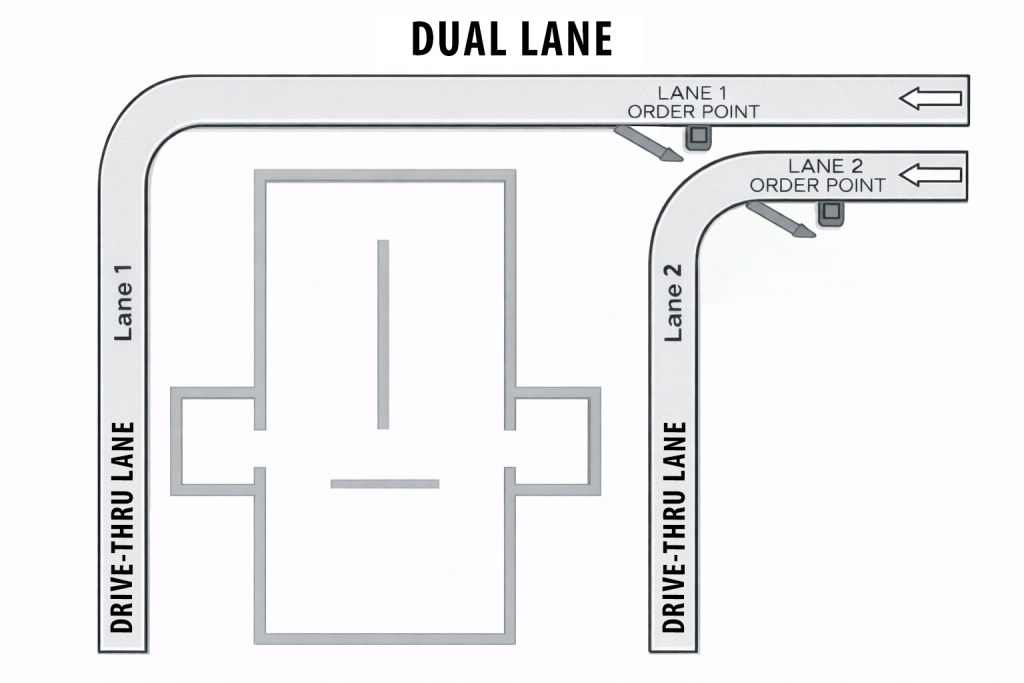
\includegraphics[width=0.65\textwidth]{./Figuras/driveThruView.png}
\caption{Esquema de un \driveThru}
\label{fig:driveThruView}
\end{figure}

Actualmente, la mayoría de las soluciones comerciales utilizadas en sistemas \driveThru{}, en particular las encargadas de la interacción entre el cliente y el personal del restaurante en el \orderPoint{}, utilizan sistemas operativos de propósito general (GPOS por sus siglas en inglés) para facilitar una rápida implementación e integración con las tecnologías de comunicación existentes. Sin embargo, a medida que aumentan los requerimientos en cuanto a confiabilidad, las características de los GPOS presentan limitaciones asociadas a la calidad, ya que no están diseñados para ejecutar tareas en un tiempo específico lo cual afecta negativamente las aplicaciones de audio en tiempo real.

Ante estas restricciones, la industria de \textit{Quick Service Restaurant} (QSR) ha empleado arquitecturas cableadas para la transmisión de datos mediante enlaces Ethernet. Este enfoque permite mantener niveles bajos de latencia y alta confiabilidad en la transmisión; no obstante, presenta limitaciones frente a los costos de instalación, mantenimiento, flexibilidad y escalabilidad de la infraestructura, lo que limita la innovación en el ecosistema.

Teniendo en cuenta este panorama, las tecnologías inalámbricas tradicionales, como Bluetooth o estándares antiguos de Wi-Fi, han sido descartadas en los ecosistemas \driveThru{} debido a que presentan dificultades en entornos con alta densidad de dispositivos o elevados niveles de interferencia electromagnética. Estas condiciones afectan negativamente las métricas críticas del sistema, como la latencia, el \textit{jitter} y la pérdida de paquetes. 

A pesar de lo anterior, el desarrollo de nuevas tecnologías y estándares como Wi-Fi 6 (IEEE 802.11ax) han hecho posible que existan nuevas oportunidades para su uso en sistemas de transmisión de audio con restricciones estrictas de latencia. Esto se ha logrado gracias a la implementación de mecanismos que mejoran el uso de los canales de radiofrecuencia en condiciones adversas, como \textit{Orthogonal Frequency Division Multiple Access} (OFDMA) y \textit{Multiple User, Multiple Input Multiple Output} (MU-MIMO).

Bajo este contexto, el objetivo principal del proyecto es desarrollar una plataforma embebida de transmisión y recepción de audio en tiempo real, denominada \textit{Audio Streaming Platform} (ASP), orientada a aplicaciones \driveThru{}, particularmente en el segmento de \orderPoint{} referenciado en la figura \ref{fig:driveThruView}. Para ello, el sistema deberá transmitir audio bidireccional con una latencia cercana a los 100 ms, lo que permite una comunicación fluida entre el cliente y el operador del restaurante incluso en entornos con altos niveles de ruido ambiental, como aquellos ubicados cerca de vías de alto tráfico vehicular.

La ASP utilizará \textit{Real-time Transport Protocol} (RTP) como protocolo de alto nivel y la transmisión de datos será sobre Wi-Fi 6, lo cual facilita la interoperabilidad con diferentes consumidores finales de audio como: operadores humanos, servicios en la nube o sistemas automatizados basados en inteligencia artificial. Adicionalmente, será posible configurar y administrar el dispositivo a través de MQTT y se utilizará la autenticación mutua basada en certificados (mTLS) para garantizar una conexión segura.

En este sentido, la arquitectura general del sistema estará compuesta por los siguientes elementos:

\begin{itemize}
\item Plataforma embebida ASP encargada de la captura, reproducción y transmisión de audio.
\item Punto de acceso Wi-Fi 6 para la interconexión de los dispositivos.
\item Unidad de procesamiento encargada de recibir y retransmitir el flujo de audio.
\item Consumidor final del audio, que podrá corresponder a un operador humano o a un sistema automatizado.
\end{itemize}

En la figura \ref{fig:diagBloques} se presenta el diagrama en bloques de la arquitectura general del sistema, en la cual la ASP establece una conexión inalámbrica con el punto de acceso Wi-Fi 6 y transmite el flujo de audio utilizando RTP hacia una unidad de procesamiento central, la cual deberá redirigir el audio hacia diferentes destinatarios. Para el desarrollo del prototipo se utilizará el kit de desarrollo \href{https://www.nordicsemi.com/Products/Development-hardware/nRF7002-DK}{nRF 7002 DK} que posee un chip dedicado a la interfaz Wi-Fi 6 y puede operar en 5 MHz o 2.4 MHz; en cuanto al desarrollo del software se empleará Zephyr RTOS.

\begin{figure}[htpb]
\centering 
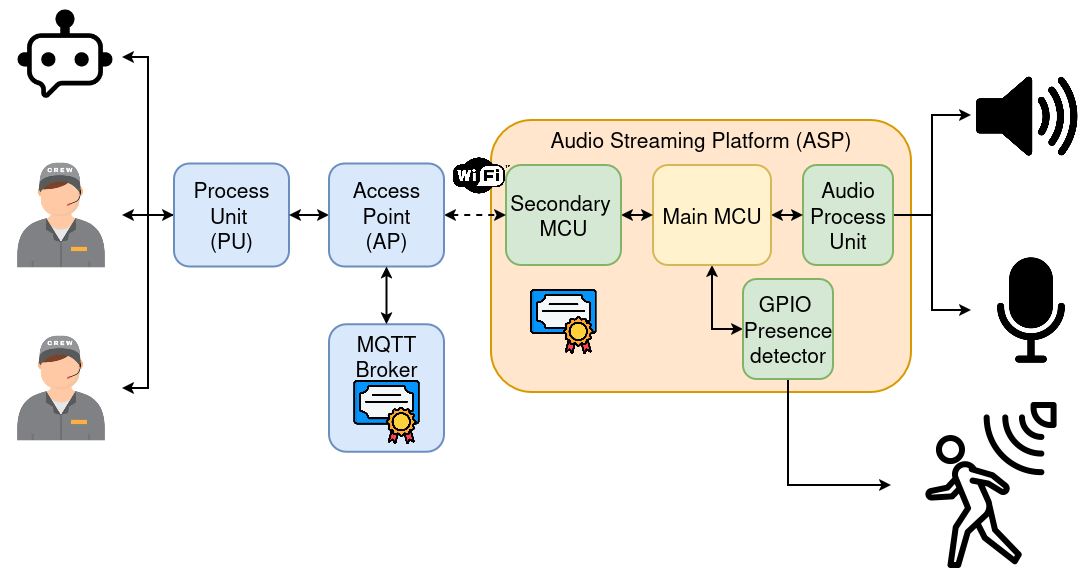
\includegraphics[width=\textwidth]{./Figuras/asp.png}
\caption{Diagrama en bloques del sistema.}
\label{fig:diagBloques}
\end{figure}


Finalmente, la propuesta de valor del proyecto consiste en ofrecer una solución flexible y escalable para sistemas \textit{Drive Thru}, lo que reduce la dependencia de una infraestructura cableada y facilita futuros cambios del sistema \driveThru{} a nivel físico. Además, el uso de protocolos estandarizados y tecnologías inalámbricas modernas mejora la interoperabilidad de la solución y habilita la integración futura con sistemas automatizados de atención al cliente.


\section{2. Identificación y análisis de los interesados}
\label{sec:interesados}


\begin{table}[ht]
\caption{Identificación de los interesados}
\label{tab:interesados}
\begin{tabularx}{\linewidth}{@{}|l|X|X|l|@{}}
\hline
\rowcolor[HTML]{C0C0C0} 
Rol           & Nombre y Apellido & Organización 	& Puesto 	\\ \hline
Cliente       & \clientename      &\empclientename	& Jurado del CESE       	\\ \hline
Responsable   & \authorname       & FIUBA        	& Alumno 	\\ \hline
Orientador    & \supname	      & \pertesupname 	& Director del Trabajo Final \\ \hline
Usuario final & Operadores de sistemas Drive Thru & Restaurantes de comida rápida & Operador del sistema       	\\ \hline
\end{tabularx}
\end{table}
 
Características de los actores:
\begin{itemize}
	\item Responsable: El \authorname{} es el encargado del diseño de la arquitectura del sistema, desarrollo del firmware embebido y quien define los requerimientos funcionales y técnicos del sistema.
	\item Orientador: El \supname{} es experto en el desarrollo e implementación de sistemas embebidos que utilizan Zephyr RTOS.
	\item Usuario final: Son los operadores de sistemas \driveThru{} y requieren una solución que permita mantener una comunicación clara y continua con los clientes, minimizando interrupciones y tiempos de espera.
\end{itemize}

\section{3. Propósito del proyecto}
\label{sec:proposito}

Desarrollar una plataforma embebida de transmisión y recepción de audio en tiempo real orientada a sistemas \driveThru{}. En primer lugar, la solución busca garantizar la comunicación bidireccional de baja latencia y calidad de audio adecuada en entornos con altos niveles de ruido. En segundo lugar, pretende reducir la dependencia de infraestructura cableada tradicional al usar Wi-Fi 6 para la transmisión del audio. En tercer lugar, se validará la viabilidad técnica del uso de protocolos estandarizados como RTP y MQTT sobre arquitecturas embebidas, para brindar una solución flexible, escalable e interoperable.

\section{4. Alcance del proyecto}
\label{sec:alcance}

El proyecto incluye:
\begin{itemize}
	\item Desarrollo de un prototipo funcional de la plataforma ASP (Audio Streaming Platform) que usará como insumo el kit de desarrollo nRF7002 DK.
	\item Implementación de transmisión de audio utilizando redes inalámbricas Wi-Fi 6 como medio principal de comunicación.
	\item Uso del protocolo RTP para el envío y recepción de audio de 16 bits en tiempo real.
	\item Desarrollo de firmware embebido para la captura, procesamiento y reproducción de audio.
	\item Integración de mecanismos de configuración y administración remota mediante MQTT.
	\item Autenticación mutua mediante certificados digitales (mTLS) para asegurar la comunicación MQTT.
	\item Evaluación de las métricas del sistema bajo las siguientes condiciones simuladas:
		\begin{itemize}
			\item Latencia de extremo a extremo.
			\item Estabilidad de la transmisión.
			\item Calidad del audio.
			\item Comportamiento en entornos con interferencia y ruido.
		\end{itemize}
	\item Documentación técnica del proyecto:
		\begin{itemize}
			\item Arquitectura de la solución.
			\item Diseño del firmware.
			\item Configuración de red.
			\item Resultados de validación.
		\end{itemize}
	\item Implementación básica de un \textit{endpoint}  RTP para recibir y enviar audio al ASP.
\end{itemize}
El presente proyecto no incluye:
\begin{itemize}
	\item Desarrollo de hardware comercial definitivo.
	\item Ejecución de algoritmos avanzados de cancelación de ruido.
	\item Integración con plataformas comerciales de punto de venta (POS por sus siglas en inglés).
	\item Desarrollo de aplicaciones móviles o interfaces gráficas avanzadas para administración del sistema.
	\item Integración con servicios \textit{cloud} externos.
	\item Desarrollo del componente de detección de presencia del cliente.
	\item Validación del sistema en condiciones reales de operación.
	
\end{itemize}



\section{5. Supuestos del proyecto}
\label{sec:supuestos}

\begin{itemize}
	\item Disponibilidad de tiempo:
		\subitem El \authorname{} cuenta con una disponibilidad de 20 horas semanales para el desarrollo del proyecto dentro de un lapso de siete meses.
		\subitem Se espera contar con la disponibilidad de \supname{} en la asesoría de consultas técnicas relacionadas con el desarrollo del firmware basado en Zephyr RTOS.
		
	\item Disponibilidad de recursos materiales:
		\subitem Se dispone de un kit de desarrollo nRF7002 DK para el prototipado de la solución y sus correspondientes pruebas.
		\subitem Se cuenta con acceso a herramientas de desarrollo adecuadas como computadoras, compiladores, depuradores y hardware de prueba.
		\subitem Se dispone de un entorno adecuado para realizar las pruebas de concepto y validación de las métricas de la solución.
		
	\item Factibilidad técnica:
		\subitem El SDK de Zephyr RTOS funcionará de manera óptima y cumple con los requisitos funcionales del proyecto.
		\subitem La red local Wi-Fi tendrá un desempeño adecuado para la transmisión de audio bidireccional con baja latencia en el entorno de pruebas.
		\subitem Los dispositivos embebidos seleccionados tendrán capacidad de procesamiento adecuada para ejecutar simultáneamente la captura, procesamiento, reproducción y transmisión de audio en tiempo real.
		\subitem El protocolo RTP podrá implementarse de manera efectiva y sin afectar la latencia general del sistema.
		\subitem La implementación de MQTT con mTLS será viable dentro de las restricciones de memoria y procesamiento del sistema embebido.
		\subitem El sistema podrá alcanzar una latencia cercana a los 100 ms en condiciones normales de operación.
		
	\item Condiciones externas:
		\subitem No existirán restricciones regulatorias que impidan el uso de redes Wi-Fi 6 y transmisión inalámbrica de audio en el entorno de desarrollo.
		\subitem No se presentarán problemas de disponibilidad de componentes electrónicos o dispositivos necesarios para el prototipado.
		\subitem El acceso a documentación técnica, SDKs y librerías necesarias para el desarrollo permanecerá disponible durante toda la ejecución del proyecto.
		
\end{itemize}


\section{6. Requerimientos}
\label{sec:requerimientos}


\begin{enumerate}
	\item Requerimientos funcionales del ASP:
		\begin{enumerate}
			\item Realizar la transmisión bidireccional (\textit{full duplex} de audio sobre RTP.
			\item Transmitir los datos a través de Wi-Fi 6.
			\item Capturar audio desde un micrófono.
			\item Reproducir audio en un parlante.			
			\item Establecer la autenticación mutua (mTLS) al conectarse al broker MQTT.
			\item Configurar los parámetros de operación a través de MQTT.
			\item La configuración remota debe incluir:
				\begin{enumerate}
					\item Identificador del dispositivo.
					\item Dirección IP o nombre del broker MQTT.
					\item Parámetros básicos de red.
					\item Parámetros asociados al flujo RTP.
				\end{enumerate}					
			\item Reintentar la conexión Wi-Fi si hay interrupciones.
			\item Reintentar la conexión con el broker MQTT si hay interrupciones.
			\item Registrar eventos básicos de funcionamiento para facilitar tareas de depuración.
		\end{enumerate}			

	\item Requerimientos no funcionales:
		\begin{enumerate}
			\item La ASP se debe implementar sobre una arquitectura embebida con soporte para Wi-Fi 6.
			\item La latencia de extremo a extremo del sistema no puede superar los 100 ms en condiciones normales de operación.
			\item El sistema debe soportar la transmisión de audio bidireccional continua sin interrupciones perceptibles durante al menos 30 minutos.
			\item La transmisión de audio debe mantener una calidad aceptable para la comunicación de voz en entornos ruidosos.
			\item El sistema debe operar correctamente bajo condiciones moderadas de interferencia inalámbrica.
			\item El firmware desarrollado debe ser modular, reutilizable y escalable para facilitar futuras extensiones.
			\item La conexión MQTT debe utilizar cifrado TLS para proteger la información transmitida.
			\item El consumo de recursos de CPU y memoria debe mantenerse dentro de las capacidades del hardware seleccionado.
			\item El sistema debe permitir la actualización de parámetros de configuración sin necesidad de recompilar el firmware.
		\end{enumerate}

	\item Requerimientos de validación:
		\begin{enumerate}
			\item Realizar pruebas de latencia extremo a extremo en la transmisión de audio.
			\item Validar el correcto funcionamiento de la transmisión RTP sobre Wi-Fi 6.
			\item Verificar la estabilidad de la comunicación inalámbrica durante transmisiones continuas.
			\item Comprobar el funcionamiento de la lógica de reconexión tanto a la red Wi-Fi como al broker MQTT.
			\item Analizar el comportamiento del dispositivo en presencia de ruido e interferencia inalambrica.
			\item Verificar que la calidad del audio transmitido sea suficiente para mantener una conversación inteligible.	
		\end{enumerate}

	\item Requerimientos de documentación:
		\begin{enumerate}
			\item Descripción de la arquitectura del ASP.
			\item Guía de instalación y configuración inicial.
			\item Especificación sobre los mensajes MQTT soportados en el sistema.
			\item Resultados de las mediciones de latencia realizadas.
		\end{enumerate}
\end{enumerate}


\section{7. Historias de usuarios (\textit{Product backlog})}
\label{sec:backlog}

Para la planificación de las historias de usuarios se tuvieron en cuenta los siguientes roles:
\begin{itemize}

	\item Administrador: es el responsable técnico encargado de instalar, configurar y realizar el mantenimiento de la plataforma ASP en las instalaciones del restaurante.
	\item Operador: corresponde al personal del restaurante que interactúa con la plataforma ASP para comunicarse con el cliente en el \driveThru.
	\item Usuario final: es el cliente que realiza el pedido a través del ASP en el \driveThru.
	\item Desarrollador: es el \authorname es encargado del diseño e implementación de la plataforma embebida.
\end{itemize}


Las historias de usuario se agruparon en torno a 4 funcionalidades y el esfuerzo que implicará cada historia se calculó con base en tres criterios:

\begin{itemize}
	\item Relevancia funcional.
	\item Dificultad técnica.
	\item Nivel de incertidumbre.
\end{itemize}

En este sentido cada criterio tiene un valor entre 1 y 3, y el esfuerzo total de cada tarea corresponde a la suma de dichos valores. Por lo tanto el puntaje mínimo es de 3 y el máximo es de 9.

\begin{enumerate}

	\item Comunicación de audio en tiempo real:

	\begin{enumerate}
			
		\item Como cliente del restaurante, quiero comunicarme de manera clara y eficiente con el personal para mantener una conversación fluida y realizar mi pedido en el menor tiempo posible. \storyPoints{}: 9 (relevancia 3, dificultad 3, incertidumbre 3).
		
		\item Como personal del restaurante, quiero que la latencia de extremo a extremo sea a lo sumo 100 ms para evitar interrupciones en la conversación con el cliente. \storyPoints{}: 8 (relevancia 2, dificultad 3, incertidumbre 3).
	
		\item Como desarrollador, quiero implementar el \textit{streaming} de audio sobre RTP para garantizar la interoperabilidad con diferentes consumidores finales. \storyPoints{}: 7 (relevancia 2, dificultad 2, incertidumbre 3).
	
	\end{enumerate}

	\item Conectividad inalámbrica:
	
		\begin{enumerate}
			\item Como administrador, quiero que el ASP se comunique utilizando Wi-Fi 6 para garantizar flexibilidad en la instalación. \storyPoints{}: 5 (relevancia 3, dificultad 1, incertidumbre 1)
			
			\item Como administrador, quiero que el dispositivo recupere automáticamente la conexión Wi-Fi en caso de alguna interrupción para garantizar la continuidad operativa. \storyPoints{}: 4 (relevancia 2, dificultad 1, incertidumbre 1).
			
			\item Como administrador, quiero validar el desempeño del sistema bajo interferencia inalámbrica moderada para asegurar un funcionamiento estable en escenarios reales. \storyPoints{}: 7 (relevancia 2, dificultad 2, incertidumbre 3).
			
			\item (Opcional) Como administrador, quiero soportar múltiples ASP conectados simultáneamente para verificar la escalabilidad de la solución. \storyPoints{}: 7 (relevancia 3, dificultad 1, incertidumbre 3).

		\end{enumerate}
		
		
	\item Configuración y seguridad:
		\begin{enumerate}
			\item Como administrador, quiero configurar el ASP remotamente a través de MQTT para modificar parámetros de operación sin acceder físicamente al hardware. \storyPoints{}: 5 (relevancia 2, dificultad 2, incertidumbre 1).
			
			\item Como administrador, quiero utilizar autenticación mutua mTLS para garantizar una comunicación segura entre el ASP y el broker MQTT. \storyPoints{}: 7 (relevancia 3, dificultad 3, incertidumbre 1).
			
			\item Como desarrollador, quiero visualizar logs básicos de operación para facilitar tareas de depuración y validación del sistema. \storyPoints{}: 4 (relevancia 2, dificultad 1, incertidumbre 1).
			
			\item (Opcional) Como administrador, quiero que el firmware del dispositivo se pueda actualizar de manera remota para simplicar el proceso de despliegue de nuevas versiones del software. \storyPoints{}: 9 (relevancia 3, dificultad 3, incertidumbre 3).
			
		\end{enumerate}			
	\item Validación y documentación:
	
		\begin{enumerate}
			\item Como desarrollador, quiero medir la latencia de extremo a extremo del sistema de una manera eficiente y escalabre para validar el cumplimiento de los requerimientos de tiempo real y garantizar que los cambios del software no afectan el desempeño del sistema. \storyPoints{}: 9 (relevancia 3, dificultad 3, incertidumbre 3).
			
			\item Como desarrollador, quiero evaluar la calidad del audio transmitido en entornos ruidosos para verificar la inteligibilidad de la comunicación. \storyPoints{}: 5 (relevancia 2, dificultad 2, incertidumbre 1).
			
			\item Como administrador, quiero recibir la documentación técnica de la arquitectura y firmware para comprender el funcionamiento interno del sistema. \storyPoints{}: 5 (relevancia 3, dificultad 1, incertidumbre 1).
			
			\item Como administrador, quiero disponer de documentación de pruebas y validaciones realizadas para verificar la confiabilidad del prototipo. \storyPoints{}: 5 (relevancia 3, dificultad 1, incertidumbre 1).
			
			\item Como administrador, quiero contar con una guía básica de instalación y puesta en marcha para facilitar el despliegue de la solución. \storyPoints{}: 5 (relevancia 3, dificultad 1, incertidumbre 1).
			
		\end{enumerate}

\end{enumerate}


\section{8. Entregables principales del proyecto}
\label{sec:entregables}

\begin{itemize}
	\item Prototipo funcional de la plataforma ASP.
	\item Código fuente del firmware basado en el kit de desarrollo nRF 7002 DK.
	\item Documentación técnica sobre los resultados de las pruebas funcionales, descripción de la arquitectura, explicación del firmware y sus componentes.
	\item Manual de usuario para la configuración a través de MQTT.
	\item Guía de puesta en marcha, en donde se indicará los requerimientos de red.
	\item Memoria del trabajo final.
\end{itemize}


\section{9. Desglose del trabajo en tareas}
\label{sec:wbs}


\begin{enumerate}
	\item Planificación del proyecto (50 h):
		\begin{enumerate}
			\item Definición requerimientos (10 h).
			\item Definición plan de trabajo (10 h).
			\item Elaboración del documento de planificación (30 h).
		\end{enumerate}

	\item Preparación del entorno de desarrollo (70 h):
		\begin{enumerate}
			\item Selección y compra de los componentes (4 h).
			\item Configuración del SDK y herramientas de compilación (4 h).
			\item Configuración del punto de acceso Wi-Fi 6 (2 h).
			\item Montaje y pruebas iniciales (30 h).
			\item Implementación básica de servidor RTP para pruebas de audio (30 h).
		\end{enumerate}	
	
	\item Desarrollo del firmware (340 h):
		\begin{enumerate}
			\item Consulta de la documentación sobre Zephyr RTOS para el manejo de nRF 7002 DK (40 h).
			\item Prueba de los ejemplos básicos del SDK para utilizar Wi-Fi (40 h).
			\item Captura del audio desde un micrófono (20 h).
			\item Reproducción de audio en un parlante (20 h).
			\item Comunicación de datos sobre Wi-Fi 6 (30 h).
			\item Reconexión automática a red Wi-Fi (10 h).
			\item Transmisión y recepción de audio sobre RTP (40 h).
			\item Implementación de cliente MQTT embebido (10 h).
			\item Configuración TLS y certificados digitales (20 h).
			\item Autenticación mutua mTLS (20 h).
			\item Configuración remota de parámetros a través de MQTT (30 h).
			\item Reconexión automática a broker MQTT (10 h).
			\item Almacenamiento persistente de la configuración (30 h).
			\item Sistema básico de logs (20 h).
		\end{enumerate}
	
	\item Pruebas y validaciones (60 h):
		\begin{enumerate}
			\item Estabilidad del audio bidireccional (10 h).
			\item Inteligibilidad del audio bidireccional (5 h).
			\item Medición de latencia extremo a extremo (10 h).
			\item Estabilidad de conexión inalámbrica (5 h).
			\item Recuperación automática de conexión (Wi-Fi, MQTT) (10 h).
			\item Interferencia inalámbrica (5 h).
			\item Comportamiento bajo carga de red (5 h).
			\item Comportamiento en entornos ruidosos (5 h).
			\item Autenticación mutua mediante mTLS (5 h).
		\end{enumerate}

	\item Documentación (80 h):
		\begin{enumerate}
			\item Arquitectura técnica del sistema (10 h).
			\item Descripción técnica del firmware (10 h).
			\item Manual de usuario (10 h).
			\item Resultados de pruebas de validación (10 h).
			\item Memoria del trabajo final (40 h).
		\end{enumerate}
\end{enumerate}

Cantidad total de horas: 600 h.


\section{10. Diagrama de Activity On Node}
\label{sec:AoN}

\begin{consigna}{red}
Armar el AoN a partir del WBS definido en la etapa anterior.

Una herramienta simple para desarrollar los diagramas es el Draw.io (\url{https://app.diagrams.net/}).
\href{https://app.diagrams.net}{Draw.io}


\begin{figure}[htpb]
\centering 
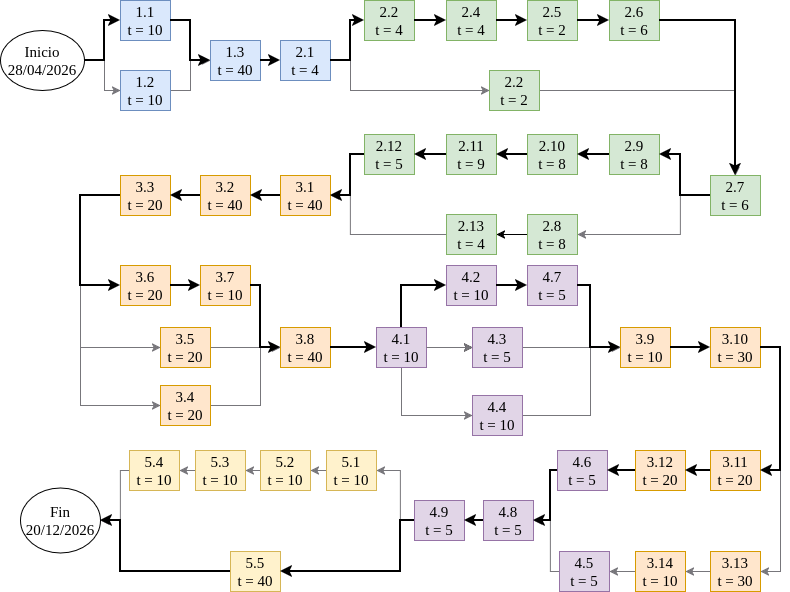
\includegraphics[width=.8\textwidth]{./Figuras/AoN.png}
\caption{Diagrama de \textit{Activity on Node}.}
\label{fig:AoN}
\end{figure}

Indicar claramente en qué unidades están expresados los tiempos.
De ser necesario indicar los caminos semi críticos y analizar sus tiempos mediante un cuadro.
Es recomendable usar colores y un cuadro indicativo describiendo qué representa cada color.

\end{consigna}

\section{11. Diagrama de Gantt}
\label{sec:gantt}

\begin{consigna}{red}
Existen muchos programas y recursos \textit{online} para hacer diagramas de Gantt, entre los cuales destacamos:

\begin{itemize}
\item Planner
\item GanttProject
\item Trello + \textit{plugins}. En el siguiente link hay un tutorial oficial: \\ \url{https://blog.trello.com/es/diagrama-de-gantt-de-un-proyecto}
\item Creately, herramienta online colaborativa. \\\url{https://creately.com/diagram/example/ieb3p3ml/LaTeX}
\item Se puede hacer en latex con el paquete \textit{pgfgantt}\\ \url{http://ctan.dcc.uchile.cl/graphics/pgf/contrib/pgfgantt/pgfgantt.pdf}
\end{itemize}

Pegar acá una captura de pantalla del diagrama de Gantt, cuidando que la letra sea suficientemente grande como para ser legible. 
Si el diagrama queda demasiado ancho, se puede pegar primero la ``tabla'' del Gantt y luego pegar la parte del diagrama de barras del diagrama de Gantt.

Configurar el software para que en la parte de la tabla muestre los códigos del EDT (WBS).\\
Configurar el software para que al lado de cada barra muestre el nombre de cada tarea.\\
Revisar que la fecha de finalización coincida con lo indicado en el Acta Constitutiva.

En la figura \ref{fig:gantt}, se muestra un ejemplo de diagrama de gantt realizado con el paquete de \textit{pgfgantt}. 
En la plantilla pueden ver el código que lo genera y usarlo de base para construir el propio.

Las fechas pueden ser calculadas utilizando alguna de las herramientas antes citadas. Sin embargo, el siguiente ejemplo
fue elaborado utilizando 
\href{https://docs.google.com/spreadsheets/d/1fBz8NhSpc4tkkhz3KjJCbh1nR_ltDkfEcZi4tZXduqs}{esta hoja de cálculo}.

Es importante destacar que el ancho del diagrama estará dado por la longitud del texto utilizado para las tareas 
(Ejemplo: tarea 1, tarea 2, etcétera) y el valor \textit{x unit}. Para mejorar la apariencia del diagrama, es necesario
ajustar este valor y, quizás, acortar los nombres de las tareas.

\begin{figure}[htpb]
  \begin{center}
    \begin{ganttchart}[
      time slot unit=day,
      time slot format=isodate,
      x unit=0.038cm,
      y unit title=0.7cm,
      y unit chart=0.6cm,
      milestone/.append style={xscale=4}
      ]{2021-03-05}{2021-12-16}
      \gantttitlecalendar*{2021-03-05}{2021-12-16}{year} \\
      \gantttitlecalendar*{2021-03-05}{2021-12-16}{month} \\
      \ganttgroup{Duración Total}{2021-03-05}{2021-12-16} \\
      %%%%%%%%%%%%%%%%%Organización
      \ganttgroup{Organización}{2021-03-05}{2021-04-16} \\
      \ganttbar{Planificación del proyecto}{2021-03-05}{2021-04-15} \\
      %%%%%%%%%%%%%%%%%Ejecución
      \ganttgroup{Ejecución}{2021-04-16}{2021-10-21} \\
      \ganttbar{Tarea 1}{2021-04-16}{2021-04-29} \\
      \ganttbar{Tarea 2}{2021-04-30}{2021-05-13} \\
      \ganttbar{Tarea 3}{2021-05-14}{2021-05-27} \\
      \ganttbar{Tarea 4}{2021-05-28}{2021-07-12} \\
      \ganttbar{Tarea 5}{2021-07-13}{2021-08-09} \\
      \ganttbar{Tarea 6}{2021-08-10}{2021-09-23} \\
      \ganttbar{Tarea 7}{2021-09-24}{2021-09-30} \\
      \ganttbar{Tarea 8}{2021-10-01}{2021-10-14} \\
      \ganttbar{Tarea 9}{2021-10-15}{2021-10-21} \\
      % %%%%%%%%%%%%%%%%%Finalización
      \ganttgroup{Finalización}{2021-10-22}{2021-12-16} \\
      \ganttbar{Memoria v1}{2021-10-22}{2021-11-04} \\
      \ganttbar{Memoria v2}{2021-11-05}{2021-11-18} \\
      \ganttbar{Memoria final}{2021-11-19}{2021-12-02} \\
      % La fecha del siguiente milestone es la fecha en que terminamos la memoria
      \ganttmilestone{Enviar memoria al director}{2021-12-02} \\
      \ganttbar{Elaborar la presentación}{2021-12-03}{2021-12-16} \\
      \ganttmilestone{Ensayo de la presentación}{2021-12-16} \\
      %%%%%%%%%%%%%%%%%%%%%%%%%%%%%%%%%%%%%%%%%%%%%%%%%%%%%%%%%%%%%%%
    \end{ganttchart}
  \end{center}
  \caption{Diagrama de gantt de ejemplo}
  \label{fig:gantt}
\end{figure}


\begin{landscape}
\begin{figure}[htpb]
\centering 
\includegraphics[height=.85\textheight]{./Figuras/Gantt-2.png}
\caption{Ejemplo de diagrama de Gantt (apaisado).} %Modificar este título acorde.
\label{fig:diagGantt}
\end{figure}

\end{landscape}

\end{consigna}


\section{12. Presupuesto detallado del proyecto}
\label{sec:presupuesto}

\begin{consigna}{red}
Si el proyecto es complejo entonces separarlo en partes:
\begin{itemize}
	\item Un total global, indicando el subtotal acumulado por cada una de las áreas.
	\item El desglose detallado del subtotal de cada una de las áreas.
\end{itemize}

IMPORTANTE: No olvidarse de considerar los COSTOS INDIRECTOS.

Incluir la aclaración de si se emplea como moneda el peso argentino (ARS) o si se usa moneda extranjera (USD, EUR, etc). Si es en moneda extranjera se debe indicar la tasa de conversión respecto a la moneda local en una fecha dada.

\end{consigna}

\begin{table}[htpb]
\centering
\begin{tabularx}{\linewidth}{@{}|X|c|r|r|@{}}
\hline
\rowcolor[HTML]{C0C0C0} 
\multicolumn{4}{|c|}{\cellcolor[HTML]{C0C0C0}COSTOS DIRECTOS} \\ \hline
\rowcolor[HTML]{C0C0C0} 
Descripción &
  \multicolumn{1}{c|}{\cellcolor[HTML]{C0C0C0}Cantidad} &
  \multicolumn{1}{c|}{\cellcolor[HTML]{C0C0C0}Valor unitario} &
  \multicolumn{1}{c|}{\cellcolor[HTML]{C0C0C0}Valor total} \\ \hline
 &
  \multicolumn{1}{c|}{} &
  \multicolumn{1}{c|}{} &
  \multicolumn{1}{c|}{} \\ \hline
 &
  \multicolumn{1}{c|}{} &
  \multicolumn{1}{c|}{} &
  \multicolumn{1}{c|}{} \\ \hline
\multicolumn{1}{|l|}{} &
   &
   &
   \\ \hline
\multicolumn{1}{|l|}{} &
   &
   &
   \\ \hline
\multicolumn{3}{|c|}{SUBTOTAL} &
  \multicolumn{1}{c|}{} \\ \hline
\rowcolor[HTML]{C0C0C0} 
\multicolumn{4}{|c|}{\cellcolor[HTML]{C0C0C0}COSTOS INDIRECTOS} \\ \hline
\rowcolor[HTML]{C0C0C0} 
Descripción &
  \multicolumn{1}{c|}{\cellcolor[HTML]{C0C0C0}Cantidad} &
  \multicolumn{1}{c|}{\cellcolor[HTML]{C0C0C0}Valor unitario} &
  \multicolumn{1}{c|}{\cellcolor[HTML]{C0C0C0}Valor total} \\ \hline
\multicolumn{1}{|l|}{} &
   &
   &
   \\ \hline
\multicolumn{1}{|l|}{} &
   &
   &
   \\ \hline
\multicolumn{1}{|l|}{} &
   &
   &
   \\ \hline
\multicolumn{3}{|c|}{SUBTOTAL} &
  \multicolumn{1}{c|}{} \\ \hline
\rowcolor[HTML]{C0C0C0}
\multicolumn{3}{|c|}{TOTAL} &
   \\ \hline
\end{tabularx}%
\end{table}


\section{13. Gestión de riesgos}
\label{sec:riesgos}

\begin{consigna}{red}
a) Identificación de los riesgos (al menos cinco) y estimación de sus consecuencias:
 
Riesgo 1: detallar el riesgo (riesgo es algo que si ocurre altera los planes previstos de forma negativa)
\begin{itemize}
	\item Severidad (S): mientras más severo, más alto es el número (usar números del 1 al 10).\\
	Justificar el motivo por el cual se asigna determinado número de severidad (S).
	\item Probabilidad de ocurrencia (O): mientras más probable, más alto es el número (usar del 1 al 10).\\
	Justificar el motivo por el cual se asigna determinado número de (O). 
\end{itemize}   

Riesgo 2:
\begin{itemize}
	\item Severidad (S): X.\\
	Justificación...
	\item Ocurrencia (O): Y.\\
	Justificación...
\end{itemize}

Riesgo 3:
\begin{itemize}
	\item Severidad (S):  X.\\
	Justificación...
	\item Ocurrencia (O): Y.\\
	Justificación...
\end{itemize}


b) Tabla de gestión de riesgos:      (El RPN se calcula como RPN=SxO)

\begin{table}[htpb]
\centering
\begin{tabularx}{\linewidth}{@{}|X|c|c|c|c|c|c|@{}}
\hline
\rowcolor[HTML]{C0C0C0} 
Riesgo & S & O & RPN & S* & O* & RPN* \\ \hline
       &   &   &     &    &    &      \\ \hline
       &   &   &     &    &    &      \\ \hline
       &   &   &     &    &    &      \\ \hline
       &   &   &     &    &    &      \\ \hline
       &   &   &     &    &    &      \\ \hline
\end{tabularx}%
\end{table}

Criterio adoptado: 

Se tomarán medidas de mitigación en los riesgos cuyos números de RPN sean mayores a...

Nota: los valores marcados con (*) en la tabla corresponden luego de haber aplicado la mitigación.

c) Plan de mitigación de los riesgos que originalmente excedían el RPN máximo establecido:
 
Riesgo 1: plan de mitigación (si por el RPN fuera necesario elaborar un plan de mitigación).
  Nueva asignación de S y O, con su respectiva justificación:
  \begin{itemize}
	\item Severidad (S*): mientras más severo, más alto es el número (usar números del 1 al 10).
          Justificar el motivo por el cual se asigna determinado número de severidad (S).
	\item Probabilidad de ocurrencia (O*): mientras más probable, más alto es el número (usar del 1 al 10).
          Justificar el motivo por el cual se asigna determinado número de (O).
	\end{itemize}

Riesgo 2: plan de mitigación (si por el RPN fuera necesario elaborar un plan de mitigación).
 
Riesgo 3: plan de mitigación (si por el RPN fuera necesario elaborar un plan de mitigación).

\end{consigna}


\section{14. Gestión de la calidad}
\label{sec:calidad}

\begin{consigna}{red}
Elija al menos diez requerimientos que a su criterio sean los más importantes/críticos/que aportan más valor y para cada uno de ellos indique las acciones de verificación y validación que permitan asegurar su cumplimiento.

\begin{itemize} 
\item Req \#1: copiar acá el requerimiento con su correspondiente número.

\begin{itemize}
	\item Verificación para confirmar si se cumplió con lo requerido antes de mostrar el sistema al cliente. Detallar.
	\item Validación con el cliente para confirmar que está de acuerdo en que se cumplió con lo requerido. Detallar. 
\end{itemize}

\end{itemize}

Tener en cuenta que en este contexto se pueden mencionar simulaciones, cálculos, revisión de hojas de datos, consulta con expertos, mediciones, etc.  

Las acciones de verificación suelen considerar al entregable como ``caja blanca'', es decir se conoce en profundidad su funcionamiento interno.  

En cambio, las acciones de validación suelen considerar al entregable como ``caja negra'', es decir, que no se conocen los detalles de su funcionamiento interno.

\end{consigna}

\section{15. Procesos de cierre}    
\label{sec:cierre}

\begin{consigna}{red}
Establecer las pautas de trabajo para realizar una reunión final de evaluación del proyecto, tal que contemple las siguientes actividades:

\begin{itemize}
	\item Pautas de trabajo que se seguirán para analizar si se respetó el Plan de Proyecto original:\\
	 - Indicar quién se ocupará de hacer esto y cuál será el procedimiento a aplicar. 
	\item Identificación de las técnicas y procedimientos útiles e inútiles que se emplearon, los problemas que surgieron y cómo se solucionaron:\\
	 - Indicar quién se ocupará de hacer esto y cuál será el procedimiento para dejar registro.
	\item Indicar quién organizará el acto de agradecimiento a todos los interesados, y en especial al equipo de trabajo y colaboradores:\\
	  - Indicar esto y quién financiará los gastos correspondientes.
\end{itemize}

\end{consigna}

\end{document}